\documentclass{article}

\usepackage{color,amsmath,amssymb,graphicx,fancyhdr,amsfonts,amsthm,algorithmic,verbatim,bbold,environ}
\usepackage{algorithm,hyperref}
\usepackage{mkolar_definitions}
\usepackage{multirow}
\usepackage{diagbox}
\usepackage{longtable,booktabs}
\usepackage[left=2cm,top=2cm,right=2cm]{geometry}
\numberwithin{algorithm}{section}

\newcommand{\tightlist}{%
  \setlength{\itemsep}{0pt}\setlength{\parskip}{0pt}}


%%%%%%%%%%%%%%%%%%%%%%%%%%%%%
\newcommand{\tta}{\theta}
\newcommand{\lag}{\left\langle}
\newcommand{\rag}{\right\rangle}
\newcommand{\lnorm}{\left\|}
\newcommand{\rnorm}{\right\|}
%%%%%%%%%%%%%%%%%%%%%%%%%%%%%



\title{CS258 Information Theory Homework 4}
\author{Zhou Litao 518030910407 F1803016}
\date{\today}
\begin{document}
\maketitle

%%%%%%%%%%%%%%%%%%%%%%%%%%%%%%%%%%%%%%%%%%
%%%%%%%%%%%%%                 %%%%%%%%%%%%
%%%%%%%%%%%%%    EXERCISE 1   %%%%%%%%%%%%
%%%%%%%%%%%%%                 %%%%%%%%%%%%
%%%%%%%%%%%%%%%%%%%%%%%%%%%%%%%%%%%%%%%%%%
\begin{exercise}[Monotonicity of entropy per element]{For a stationary stochastic process $X_{1}, X_{2}, \ldots, X_{n},$ show that
  $$
  \begin{aligned}
  \frac{H\left(X_{1}, X_{2}, \ldots, X_{n}\right)}{n} & \leq \frac{H\left(X_{1}, X_{2}, \ldots, X_{n-1}\right)}{n-1} \\
  \frac{H\left(X_{1}, X_{2}, \ldots, X_{n}\right)}{n} & \geq H\left(X_{n} | X_{n-1}, \ldots, X_{1}\right)
  \end{aligned}
  $$}
  \begin{proof}
  \par{~}

  We first prove the second statement by properties of stationary process.

  \begin{equation}\begin{aligned}
    H\left(X_{1}, \cdots, X_{n}\right) &=\sum_{i=1}^{n} H\left(X_{i} | X_{i-1}, \cdots X_{2}, X_{1}\right) \\
    & \geqslant \sum_{i=1}^{n} H\left(X_{i} | X_{i-1}, X_{i-2}, \cdots, X_{n-i+1}\right) \\
    &=\sum_{i=1}^{n} H\left(X_{n} | X_{n-1}, \cdots, X_{2}, X_{1}\right) \\
    &=n H\left(X_{n} | X_{1}, X_{2}, \cdots, X_{n-1}\right)
    \end{aligned}\label{eqn:ex1}\end{equation}

    By Equation \ref{eqn:ex1} and entropy equalities we can prove the first statement.

  \begin{equation}\begin{aligned}
    (n-1) H\left(X_{1}, \cdots, X_{n}\right) & \leqslant n H\left(X_{1}, \cdots, X_{n}\right)-H\left(X_{1}, \cdots, X_{n}\right) \\
    & \leqslant n\left[H\left(X_{1}, \cdots, X_{n}\right)-H\left(X_{n}|X_{1}, \cdots, X_{n-1}\right)\right]\\
    &=n H\left(X_{1}, \cdots, X_{n-1}\right)
    \end{aligned}\end{equation}


  \end{proof}
  \label{ex1}
\end{exercise}

%%%%%%%%%%%%%%%%%%%%%%%%%%%%%%%%%%%%%%%%%%
%%%%%%%%%%%%%                 %%%%%%%%%%%%
%%%%%%%%%%%%%    EXERCISE 2   %%%%%%%%%%%%
%%%%%%%%%%%%%                 %%%%%%%%%%%%
%%%%%%%%%%%%%%%%%%%%%%%%%%%%%%%%%%%%%%%%%%
\begin{exercise}[Initial conditions]{ Show, for a Markov chain, that
  $$
  H\left(X_{0} | X_{n}\right) \geq H\left(X_{0} | X_{n-1}\right)
  $$
  Thus, initial conditions $X_{0}$ become more difficult to recover as the future $X_{n}$ unfolds.}
  \begin{proof}
  For Markov Chain, we have $p(x_0|x_n,x_{n-1}) = p(x_0|x_{n-1})$. Hence
  \begin{equation}
    \begin{aligned}
      H(X_0|X_n,X_{n-1}) &= -\sum_{x_n,x_{n-1}} p(x_n,x_{n-1}) \sum_{x_0} p(x_0|x_n,x_{n-1}) \log    p(x_0|x_n,x_{n-1}) \\
      &= -\sum_{x_{n-1}} \left( \sum_{x_{n}} p(x_n,x_{n-1}) \right) \sum_{x_0} p(x_0|x_{n-1}) \log    p(x_0|x_{n-1})\\
      &= -\sum_{x_{n-1}} p(x_{n-1}) \sum_{x_0} p(x_0|x_{n-1}) \log    p(x_0|x_{n-1}) = H(X_0|X_{n-1})
    \end{aligned}
  \end{equation}
  Since condition reduce entropy, we have $  H(X_0|X_{n-1}) = H(X_0|X_n,X_{n-1}) \le  H(X_0|X_n) $
  \end{proof}
  \label{ex2}
\end{exercise}

%%%%%%%%%%%%%%%%%%%%%%%%%%%%%%%%%%%%%%%%%%
%%%%%%%%%%%%%                 %%%%%%%%%%%%
%%%%%%%%%%%%%    EXERCISE 3   %%%%%%%%%%%%
%%%%%%%%%%%%%                 %%%%%%%%%%%%
%%%%%%%%%%%%%%%%%%%%%%%%%%%%%%%%%%%%%%%%%%
\begin{exercise}[The past has little to say about the future]{For a stationary stochastic process $X_{1}, X_{2}, \ldots, X_{n}, \ldots,$ show that
  $$
  \lim _{n \rightarrow \infty} \frac{1}{2 n} I\left(X_{1}, X_{2}, \ldots, X_{n} ; X_{n+1}, X_{n+2}, \ldots, X_{2 n}\right)=0
  $$}
  \begin{proof} First Note that
    \begin{equation}
      I\left(X_{1}, X_{2}, \ldots, X_{n} ; X_{n+1}, X_{n+2}, \ldots, X_{2 n}\right) = H(X_1,\ldots,X_n) - H(X_{n+1},\ldots,X_{2n}|X_1,\ldots,X_n)
    \end{equation}
    By definition of entropy rate we know that $$\frac{1}{2}\sum_{i=1}^{n} H(X_1,\ldots,X_n) \rightarrow H(\mathcal{X})$$



  \end{proof}
  \label{ex3}
\end{exercise}


%%%%%%%%%%%%%%%%%%%%%%%%%%%%%%%%%%%%%%%%%%
%%%%%%%%%%%%%                 %%%%%%%%%%%%
%%%%%%%%%%%%%    EXERCISE 4   %%%%%%%%%%%%
%%%%%%%%%%%%%                 %%%%%%%%%%%%
%%%%%%%%%%%%%%%%%%%%%%%%%%%%%%%%%%%%%%%%%%
\begin{exercise}[Entropy rate]{ Let $\left\{X_{i}\right\}$ be a discrete stationary stochastic process with entropy rate $H(\mathcal{X}) .$ Show that
  $$
  \frac{1}{n} H\left(X_{n}, \ldots, X_{1} | X_{0}, X_{-1}, \ldots, X_{-k}\right) \rightarrow H(\mathcal{X})
  $$
  for $k=1,2, \ldots$}
  \begin{proof}
  \begin{equation}
      H\left(X_{n}, \ldots, X_{1} | X_{0}, X_{-1}, \ldots, X_{-k}\right) = \sum_{i=1}^{n} H(X_i|X_{i-1},\ldots,X_{-k})
  \end{equation}
  Note that $$H'(X) = \lim_{n\rightarrow \infty}H(X_n|X_{n-1},ldots,X_1) = \lim_{n\rightarrow \infty}H(X_n|X_{n-1},\ldots,X_{-k})$$
  We already know that $H'(X)\rightarrow H(\mathcal{X})$.

  By Cesaro Mean, $$
  \frac{1}{n} H\left(X_{n}, \ldots, X_{1} | X_{0}, X_{-1}, \ldots, X_{-k}\right) \rightarrow H(\mathcal{X})
  $$
  \end{proof}
  \label{ex4}
\end{exercise}


%%%%%%%%%%%%%%%%%%%%%%%%%%%%%%%%%%%%%%%%%%
%%%%%%%%%%%%%                 %%%%%%%%%%%%
%%%%%%%%%%%%%    EXERCISE 5   %%%%%%%%%%%%
%%%%%%%%%%%%%                 %%%%%%%%%%%%
%%%%%%%%%%%%%%%%%%%%%%%%%%%%%%%%%%%%%%%%%%
\begin{exercise}[Markov’s inequality and Chebyshev’s inequality]{\par{~}
  \begin{enumerate}
    \item (Markov's inequality) For any nonnegative random variable $X$ and any $t>0,$ show that\begin{equation}\operatorname{Pr}\{X \geq t\} \leq \frac{E X}{t}\end{equation} Exhibit a random variable that achieves this inequality with equality. 
    \item (Chebyshev's inequality) Let $Y$ be a random variable with mean $\mu$ and variance $\sigma^{2} .$ By letting $X=(Y-\mu)^{2},$ show that for any $\epsilon>0$
    \begin{equation}
      \operatorname{Pr}\{|Y-\mu|>\epsilon\} \leq \frac{\sigma^{2}}{\epsilon^{2}}
    \end{equation}
    \item (Weak law of large numbers) Let $Z_{1}, Z_{2}, \ldots, Z_{n}$ be a sequence of i.i.d. random variables with mean $\mu$ and variance $\sigma^{2} .$ Let $\bar{Z}_{n}=\frac{1}{n} \sum_{i=1}^{n} Z_{i}$ be the sample mean. Show that
  \begin{equation}\operatorname{Pr}\left\{\left|\bar{Z}_{n}-\mu\right|>\epsilon\right\} \leq \frac{\sigma^{2}}{n \epsilon^{2}}\end{equation}
    Thus, $\operatorname{Pr}\left\{\left|\bar{Z}_{n}-\mu\right|>\epsilon\right\} \rightarrow 0$ as $n \rightarrow \infty .$ This is known as the weak law of large numbers.
  \end{enumerate}}
  \begin{proof}
  \par{~}
  \begin{enumerate}
    \item {
      Note that for any $t$,
      \begin{equation}
        t \cdot 1_{\left\{X\ge t\right\}} \le X
      \end{equation}
      By taking expectation at both sides we have
      \begin{equation}
        E(1_{\left\{X\ge t\right\}}) = \Pr (X\ge t) \le \frac{EX}{t}
      \end{equation}
    }
    \item {
      Note $EX = DY =\sigma^2$. By letting $X = (Y-\mu)^2$ and $t = \epsilon^2$ in the Markov inequality, we can derive that
    \begin{equation}\operatorname{Pr}\left\{\left|\bar{Z}_{n}-\mu\right|>\epsilon\right\} \leq \frac{\sigma^{2}}{n \epsilon^{2}}\end{equation}
    }
    \item {
      Note $E\bar{Z_n} = \mu$ and $D\bar{Z_n} = \frac{1}{n^2} \sum_{i=1}^n DZ_i = \frac{\sigma^2}{n}$. By applying Chebyshev's inequality on $\bar{Z_n}$ we have
    \begin{equation}\operatorname{Pr}\left\{\left|\bar{Z}_{n}-\mu\right|>\epsilon\right\} \leq \frac{\sigma^{2}}{n \epsilon^{2}}\end{equation}
    }
  \end{enumerate}
  \end{proof}
  \label{ex5}
\end{exercise}

%%%%%%%%%%%%%%%%%%%%%%%%%%%%%%%%%%%%%%%%%%
%%%%%%%%%%%%%                 %%%%%%%%%%%%
%%%%%%%%%%%%%    EXERCISE 6   %%%%%%%%%%%%
%%%%%%%%%%%%%                 %%%%%%%%%%%%
%%%%%%%%%%%%%%%%%%%%%%%%%%%%%%%%%%%%%%%%%%
\begin{exercise}[Piece of cake]{ A cake is sliced roughly in half, the largest piece being chosen each time, the other pieces discarded. We will assume that a random cut creates pieces of proportions
  $$
  P=\left\{\begin{array}{ll}
  \left(\frac{2}{3}, \frac{1}{3}\right) & \text { with probability } \frac{3}{4} \\
  \left(\frac{2}{5}, \frac{3}{5}\right) & \text { with probability } \frac{1}{4}
  \end{array}\right.
  $$
  Thus, for example, the first cut (and choice of largest piece) may result in a piece of size $\frac{3}{5} .$ Cutting and choosing from this piece might reduce it to size $\left(\frac{3}{5}\right)\left(\frac{2}{3}\right)$ at time $2,$ and so on. How large, to first order in the exponent, is the piece of cake after $n$ cuts?}
  \begin{solution}
  Let $C_1, C_2, \ldots, C_n$ denote the choice of each cut. Then after $n$ cuts, the size of the cake $W_n = \prod_{i=1}^n C_i$. By taking the logarithm at the equation, we have $\log W_n = \sum_{i=1}^n \log C_i$. Since $C_i$s are i.i.d., we can apply the law of large numbers as follows.
  \begin{equation}
    \lim_{n\rightarrow\infty}\frac{1}{n} \log W_n = E(\log C) = \frac{3}{4}\log \frac{2}{3} + \frac{1}{4} \log \frac{3}{5} \approx -0.494
  \end{equation}
  Note that the equation above indicates that
  \begin{equation}
    \begin{aligned}
      \frac{1}{n} \log W_n &= -0.494 + o(1)
      W_n &= 2^{-0.494t +o(n)}
    \end{aligned}
  \end{equation}
  So the first order in the exponent is $\frac{3}{4}\log \frac{2}{3} + \frac{1}{4} \log \frac{3}{5} \approx -0.494$.
  \end{solution}
  \label{ex6}
\end{exercise}

%%%%%%%%%%%%%%%%%%%%%%%%%%%%%%%%%%%%%%%%%%
%%%%%%%%%%%%%                 %%%%%%%%%%%%
%%%%%%%%%%%%%    EXERCISE 7   %%%%%%%%%%%%
%%%%%%%%%%%%%                 %%%%%%%%%%%%
%%%%%%%%%%%%%%%%%%%%%%%%%%%%%%%%%%%%%%%%%%
\begin{exercise}[AEP]{ Let $X_{i}$ be iid $\sim p(x), x \in\{1,2, \ldots, m\} .$ Let $\mu=E X$ and $H=-\sum p(x) \log p(x) .$ Let $A^{n}=\left\{x^{n} \in \mathcal{X}^{n}: |-\frac{1}{n} \log p\left(x^{n}\right)-\right.$
  $H | \leq \epsilon\} .$ Let $B^{n}=\left\{x^{n} \in \mathcal{X}^{n}:\left|\frac{1}{n} \sum_{i=1}^{n} X_{i}-\mu\right| \leq \epsilon\right\}$
  \begin{enumerate}
    \item Does $\operatorname{Pr}\left\{X^{n} \in A^{n}\right\} \longrightarrow 1 ?$
    \item Does $\operatorname{Pr}\left\{X^{n} \in A^{n} \cap B^{n}\right\} \longrightarrow 1 ?$
    \item Show that $\left|A^{n} \cap B^{n}\right| \leq 2^{n(H+\epsilon)}$ for all $n$
    \item Show that $\left|A^{n} \cap B^{n}\right| \geq\left(\frac{1}{2}\right) 2^{n(H-\epsilon)}$ for $n$ sufficiently large.
  \end{enumerate}}
  \begin{solution}
  \par{~}
  \begin{enumerate}
    \item {
      Yes. By the Large Number Law,
      \begin{equation}
        - \frac{1}{n}\log p(x^n) = - \frac{1}{n} \sum_{i=1}^{n} \log p(X_i) \rightarrow H(X) \text{\quad in probability}
      \end{equation}
      , which implies that
      \begin{equation}
        \Pr \left\{X^n \in A^n \right\} = \Pr \left\{ | -\frac{1}{n} \log p\left(x^{n}\right)-H | \leq \epsilon \right\} \rightarrow 1
      \end{equation}
      }
    \item {
      Yes. Part (1) implies that $\lim_{n\rightarrow\infty} \Pr \left\{X^n \in A^n \right\} = 1$.

      By strong law of large number we have $\lim_{n\rightarrow\infty} \Pr \left\{X^n \in B^n \right\} = 1$

      For arbitrary $\delta > 0$, there exists $N_1$, such that  $\Pr \left\{X^n \in A^n \right\} > 1 - \frac{\delta}{2}$ for all $n>N_1$, and there exists $N_2$, such that  $\Pr \left\{X^n \in B^n \right\} > 1 - \frac{\delta}{2}$ for all $n>N_2$.
      We take $N = \max \left\{N_1,N_2\right\}$, for any $n>N$, we have
      \begin{equation}
        \begin{aligned}
          \Pr \left\{X^{n} \in A^{n} \cap B^{n}\right\} &= \Pr \left\{X^n \in A^n \right\} +  \Pr \left\{X^n \in B^n \right\} - \Pr \left\{X^n \in A^n \cup B^n \right\}\\
          & > 1 - \frac{\delta}{2} + 1 - \frac{\delta}{2} - 1 = 1 - \delta
        \end{aligned}
      \end{equation}
      , which indicates that $\Pr \left\{X^{n} \in A^{n} \cap B^{n}\right\} \rightarrow 1$
    }
    \item {
      From $x^n\in A^n$ we know that
      \begin{equation}
        2^{-n(H+\epsilon)} \le p(x^n) \le 2^{-n(H-\epsilon)}
      \end{equation}
      \begin{equation}
        \begin{aligned}
          1 &= \sum_{x^n\in \mathcal{x}^n} p(x) \\
          &\ge \sum_{x^n\in A^n \cap B^n} p(x) \\
          &\ge 2^{-n(H(X)+\epsilon)} |A^n\cap B^n|
        \end{aligned}
      \end{equation}
      It follows that $\left|A^{n} \cap B^{n}\right| \leq 2^{-n(H+\epsilon)}$.
    }
    \item {
      From $\Pr \left\{X^n \in A^n \cap B^n \right\} \rightarrow 1$, we take $\delta = \frac{1}{2}$, then there exists sufficiently large $n$, such that
      \begin{equation}
        \begin{aligned}
          \frac{1}{2} &\le \Pr (X^n \in A^n \cap B^n) \\
          &\le \sum_{x^n \in A^n \cap B^n} p(x^n) \\
          &\le |A^n\cap B^n| 2^{-n(H(X)-\epsilon)}
        \end{aligned}
      \end{equation}
      It follows that $\left|A^{n} \cap B^{n}\right| \geq \left( \frac{1}{2}\right) 2^{-n(H-\epsilon)}$.
    }
  \end{enumerate}
  \end{solution}
  \label{ex7}
\end{exercise}

%%%%%%%%%%%%%%%%%%%%%%%%%%%%%%%%%%%%%%%%%%
%%%%%%%%%%%%%                 %%%%%%%%%%%%
%%%%%%%%%%%%%    EXERCISE 8   %%%%%%%%%%%%
%%%%%%%%%%%%%                 %%%%%%%%%%%%
%%%%%%%%%%%%%%%%%%%%%%%%%%%%%%%%%%%%%%%%%%
\begin{exercise}[Doubly stochastic matrices]{$\quad$ An $n \times n$ matrix $P=\left[P_{i j}\right]$ is said to be doubly stochastic if $P_{i j} \geq 0$ and $\sum_{j} P_{i j}=1$ for all $i$ and $\sum_{i} P_{i j}=1$ for all $j .$ An $n \times n$ matrix $P$ is said to be a permutation matrix if it is doubly stochastic and there is precisely one $P_{i j}=1$ in each row and each column. It can be shown that every doubly stochastic matrix can be written as the convex combination of permutation matrices.
  \begin{enumerate}
    \item Let $\mathbf{a}^{t}=\left(a_{1}, a_{2}, \ldots, a_{n}\right), a_{i} \geq 0, \sum a_{i}=1,$ be a probability vector. Let $\mathbf{b}=\mathbf{a} P,$ where $P$ is doubly stochastic. Show that $\mathbf{b}$ is a probability vector and that $H\left(b_{1}, b_{2}, \ldots, b_{n}\right) \geq H\left(a_{1}, a_{2}, \ldots, a_{n} \right)$. Thus, stochastic mixing increases entropy.
    \item Show that a stationary distribution $\mu$ for a doubly stochastic matrix $P$ is the uniform distribution.
    \item Conversely, prove that if the uniform distribution is a stationary distribution for a Markov transition matrix $P,$ then $P$ is doubly stochastic.
  \end{enumerate}}
  \begin{proof}
  \par{~}
  \begin{enumerate}
    \item {
      From $\mathbf{b} = \mathbf{a}P$ we know that
      \begin{equation}
        b_j = \sum_{i=1}^{m} a_i p_{ij}
      \end{equation}
      Then we have.
      \begin{equation}
        \begin{aligned}
          H(\mathbf{b}) - H(\mathbf{a}) &= - \sum_{j=1}^{m} \left(\sum_{i=1}^{m} a_i p_{ij}\right) \log  b_j + \sum_{i=1}^{m} a_i \log a_i \\
          &= - \sum_{i=1}^{m} a_i \left(\sum_{j=1}^{m} p_{ij}\log  b_j \right)+ \sum_{i=1}^{m} a_i \left(\sum_{j=1}^{m} p_{ij} \log a_i \right) \\
          &= \sum_{i=1}^{m} \sum_{j=1}^{m} a_i  p_{ij}\log \frac{a_i}{b_j} \\
          &= \sum_{i=1}^{m} \sum_{j=1}^{m} b_j  p_{ij} \left(\frac{a_i}{b_j} \log \frac{a_i}{b_j} \right) \\
          &\ge \left(\sum_{i=1}^{m} \sum_{j=1}^{m} b_j  p_{ij} \frac{a_i}{b_j} \right) \log \left(\sum_{i=1}^{m} \sum_{j=1}^{m} b_j  p_{ij} \frac{a_i}{b_j} \right) \\
          &= \left(\sum_{i=1}^{m} \sum_{j=1}^{m} p_{ij} a_i\right) \log \left(\sum_{i=1}^{m} \sum_{j=1}^{m} p_{ij} a_i\right) = 1 \cdot \log 1 = 0
        \end{aligned}
      \end{equation}
    }
    \item {
     By condition we have $\mu_i = \frac{1}{m}$ for any $i$. Since for any $j$, 
     \begin{equation}
      \sum_{i=1}^{m} \mu_i p_{ij} = \frac{1}{m} \sum_{i=1}^{m} p_{ij} = \frac{1}{m} = \mu_i
     \end{equation}
     We have that $\mathbf{\mu} P = \mathbf{\mu}$. The uniform distribution is a stationary distribution for a doubly stochastic matrix.
    }
    \item {
      From $\mathbf{\mu} P = \mathbf{\mu}$ and $\mu = \frac{1}{m}$, we know that
      \begin{equation}
        \sum_{i=1}^{m} \frac{1}{m} p_{ij} = \frac{1}{m}
       \end{equation}
      holds for any $j$, which implies
      \begin{equation}
        \sum_{i=1}^{m} p_{ij} = 1 \text{\quad for any} j
      \end{equation}
      Then $P$ is doubly stochastic.
    }
  \end{enumerate}
  \end{proof}
  \label{ex8}
\end{exercise}

%%%%%%%%%%%%%%%%%%%%%%%%%%%%%%%%%%%%%%%%%%
%%%%%%%%%%%%%                 %%%%%%%%%%%%
%%%%%%%%%%%%%    EXERCISE 9   %%%%%%%%%%%%
%%%%%%%%%%%%%                 %%%%%%%%%%%%
%%%%%%%%%%%%%%%%%%%%%%%%%%%%%%%%%%%%%%%%%%
\begin{exercise}[Shuffes increase entropy]{ Argue that for any distribution on shuffles $T$ and any distribution on card positions $X$ that
  $$
  \begin{aligned}
  H(T X) & \geq H(T X | T) \\
  &=H\left(T^{-1} T X | T\right) \\
  &=H(X | T) \\
  &=H(X)
  \end{aligned}
  $$
  if $X$ and $T$ are independent.}
  \begin{proof} The first line holds because condition reduces entropy. The second line holds since $T^{-1}$ can be given by the condition $T$. The last line holds if $X$ and $T$ are independent, which finishes the proof.
  \end{proof}
  \label{ex9}
\end{exercise}

%%%%%%%%%%%%%%%%%%%%%%%%%%%%%%%%%%%%%%%%%%
%%%%%%%%%%%%%                 %%%%%%%%%%%%
%%%%%%%%%%%%%    EXERCISE 10  %%%%%%%%%%%%
%%%%%%%%%%%%%                 %%%%%%%%%%%%
%%%%%%%%%%%%%%%%%%%%%%%%%%%%%%%%%%%%%%%%%%
\begin{exercise}[Entropy rates of Markov chains]{ \par{~}
  \begin{enumerate}
    \item Find the entropy rate of the two-state Markov chain with transition matrix
    $$
    P=\left[\begin{array}{cc}
    1-p_{01} & p_{01} \\
    p_{10} & 1-p_{10}
    \end{array}\right]
    $$
    \item What values of $p_{01}, p_{10}$ maximize the entropy rate?
    \item Find the entropy rate of the two-state Markov chain with transition matrix
    $$
    P=\left[\begin{array}{cc}
    1-p & p \\
    1 & 0
    \end{array}\right]
    $$
    \item Find the maximum value of the entropy rate of the Markov chain of part (c). We expect that the maximizing value of $p$ should be less than $\frac{1}{2},$ since the 0 state permits more information to be generated than the 1 state.
    \item Let $N(t)$ be the number of allowable state sequences of length $t$ for the Markov chain of part (c). Find $N(t)$ and calculate
    $$
    H_{0}=\lim _{t \rightarrow \infty} \frac{1}{t} \log N(t)
    $$
  \end{enumerate}
  [Hint: Find a linear recurrence that expresses $N(t)$ in terms of $N(t-1)$ and $N(t-2) .$ Why is $H_{0}$ an upper bound on the entropy rate of the Markov chain? Compare $H_{0}$ with the maximum entropy found in part (d). $]$}
  \begin{solution}
  \par{~}
  \begin{enumerate}
    \item {
      We first calculate the stationary distribution $\mathbf{\mu}$.
      \begin{equation}
        \left\{\begin{array}{c}
          \mathbf{\mu}P = \mathbf{\mu} \\
          \mathbf{\mu} \mathbf{1}^T = 1
        \end{array}\right. \Rightarrow \mu = \left[\frac{p_{10}}{p_{01}+p_{10}}, \frac{p_{01}}{p_{01}+p_{10}}\right]
      \end{equation}
      By the entropy rate of Markov Chain,
      \begin{equation}
        \begin{aligned}
          H(\mathcal{X}) &= \sum_{i=1,2} \mu_i \left(\sum_{j=1,2} - p_{ij} \log {p_{ij}}\right) \\
          &= \frac{p_{10}H(p_{01})+p_{01}H(p_{10})}{p_{01}+p_{10}}
        \end{aligned}
      \end{equation}
    }
    \item {
      Note that the entropy is upper bounded by its alphabet, since
      \begin{equation}
        \frac{1}{n} H\left(X_{1}, X_{2}, \ldots, X_{n}\right) \le \frac{1}{n} \log |\mathcal{X}|^n = \log |\mathcal{X}|
      \end{equation}
      Hence the maximal entropy rate for this problem is $\log 2 = 1$. This can be obtained when $p_{01} = p_{10} = \frac{1}{2}$, where
      \begin{equation}
        \begin{aligned}
          H(\mathcal{X}) &= \frac{p_{10}H(p_{01})+p_{01}H(p_{10})}{p_{01}+p_{10}} \\
          &= \frac{1}{2} + \frac{1}{2}  = 1
        \end{aligned}
      \end{equation}
      Therefore, $p_{01} = p_{10} = \frac{1}{2}$ maximize the entropy rate.
    }
    \item {
      We first calculate the stationary distribution $\mathbf{\mu}$.
      \begin{equation}
        \left\{\begin{array}{c}
          \mathbf{\mu}P = \mathbf{\mu} \\
          \mathbf{\mu} \mathbf{1}^T = 1
        \end{array}\right. \Rightarrow \mu = \left[\frac{1}{p+1}, \frac{p}{p+1}\right]
      \end{equation}
      By the entropy rate of Markov Chain,
      \begin{equation}
        \begin{aligned}
          H(\mathcal{X}) &= \sum_{i=1,2} \mu_i \left(\sum_{j=1,2} - p_{ij} \log {p_{ij}}\right) \\
          &= \frac{-p\log p -(1-p)\log (1-p)}{p+1}
        \end{aligned}
      \end{equation}
    }
    \item { We take the derivative of $H(\mathcal{X})$.
    \begin{equation}
        \frac{d H(\mathcal{X})}{dp} = \frac{\log(1-p) -\log p+\log(1-p)}{(p+1)^2} := 0 \quad 
        \Rightarrow \quad p =  \frac{3- \sqrt{5}}{2}
    \end{equation}
    The maximal entropy rate is $\log \frac{1+\sqrt{5}}{2} \approx 0.6942$.
    }
    \item {
      The transition matrix implies that there is no possibility that the last state is 1 with the last but one state to be 1. We can calculate the $N(t)$ recursively. If the last state is 0, the previous state possibilities add up to $N(t-1)$. If the last state is 1, however, the last but one state can only be 0. Then all the previous state possibilities will add up to $N(t-2)$. Further more, we can manually check the initial length that $N(1) = 2$, $N(2) = 3$. Now we have 
      \begin{equation}
        N(t) = N(t-1) + N(t-2)
      \end{equation}
      By solving the characteristic equation we know that $N(t)$ must be in the form like
      \begin{equation}
        N(t) = C_1 (\frac{1+\sqrt{5}}{2})^n + C_2 (\frac{1-\sqrt{5}}{2})^t
      \end{equation}
      Then
      \begin{equation}
        \begin{aligned}
          H_{0} &=\lim _{t \rightarrow \infty} \frac{1}{t} \log N(t) \\
          &= \lim _{t \rightarrow \infty} \frac{1}{t} \log \left(C_1 (\frac{1+\sqrt{5}}{2})^t + C_2 (\frac{1-\sqrt{5}}{2})^t\right) \\
          &= \lim _{t \rightarrow \infty} \frac{1}{t} \log C_1 (\frac{1+\sqrt{5}}{2})^t \\
          &= \lim _{t \rightarrow \infty} \frac{1}{t} t \log \frac{1+\sqrt{5}}{2} = \log \frac{1+\sqrt{5}}{2}
        \end{aligned}
      \end{equation}
      We find that $H_0$ is the upper bound of the entropy rate, and can be obtained with the maximum entropy found in pard (d). This is because by the property of entropy,
      \begin{equation}
        H\left(X_{1}, X_{2}, \ldots, X_{n}\right) \le \log |X_{1}, X_{2}, \ldots, X_{n}| = N(t)
      \end{equation}
    }
  \end{enumerate}
  \end{solution}
  \label{ex10}
\end{exercise}

%%%%%%%%%%%%%%%%%%%%%%%%%%%%%%%%%%%%%%%%%%
%%%%%%%%%%%%%                 %%%%%%%%%%%%
%%%%%%%%%%%%%    EXERCISE 11  %%%%%%%%%%%%
%%%%%%%%%%%%%                 %%%%%%%%%%%%
%%%%%%%%%%%%%%%%%%%%%%%%%%%%%%%%%%%%%%%%%%
\begin{exercise}[Maximal entropy graphs]{Consider a random walk on a connected graph with four edges.
  \begin{enumerate}
    \item Which graph has the highest entropy rate?
    \item Which graph has the lowest?
  \end{enumerate}}
  \begin{solution} In a random walk, the next vertex will be arbitrarily chosen from the adjancent vertices of the current vertex. That is to say, all the edges are given the same weight.

    We can formulate this problem as follows. By the inclusion-exclusion principle, there are at most 5 vertices in the graph given four edges. Their adjancent relation can be represented in a $5\times 5$ 0-1 matrix$W$, where $W_{i j} = 0$ or $1$ and $W_{i j}=W_{j i}$.

    Then the transition probability matrix $P$ and the stationary distribution$\mu$ can be calculated.
    \begin{equation}P_{i j}=\frac{W_{i j}} {\sum_{k} W_{i k}}
    \label{trans}\end{equation}
    \begin{equation}\mu_{i}=\frac{W_{i}}{2 W}\label{mu}\end{equation}

      where $W_{i}=\sum_{j} w_{i j}$ and $W=\sum_{i} \frac{W_{i}}{2}$
  
      Then the entropy rate can be calculated as
      \begin{equation}\begin{aligned}
        H(\mathcal{X})&=H\left(X_{2} | X_{1}\right) \\
        &= H(X_2,X_1) - H(X_1)\\
        &= H(\frac{1}{8},\frac{1}{8},\ldots,\frac{1}{8}) - H(\mu) \\
        &= 3 - H(\mu)
      \end{aligned}\end{equation}
      
      For 4 edges, there are five possible graphs, as has been shown in Figure \ref{fig:ex11}.

      \begin{figure}[htbp]
        \centering
        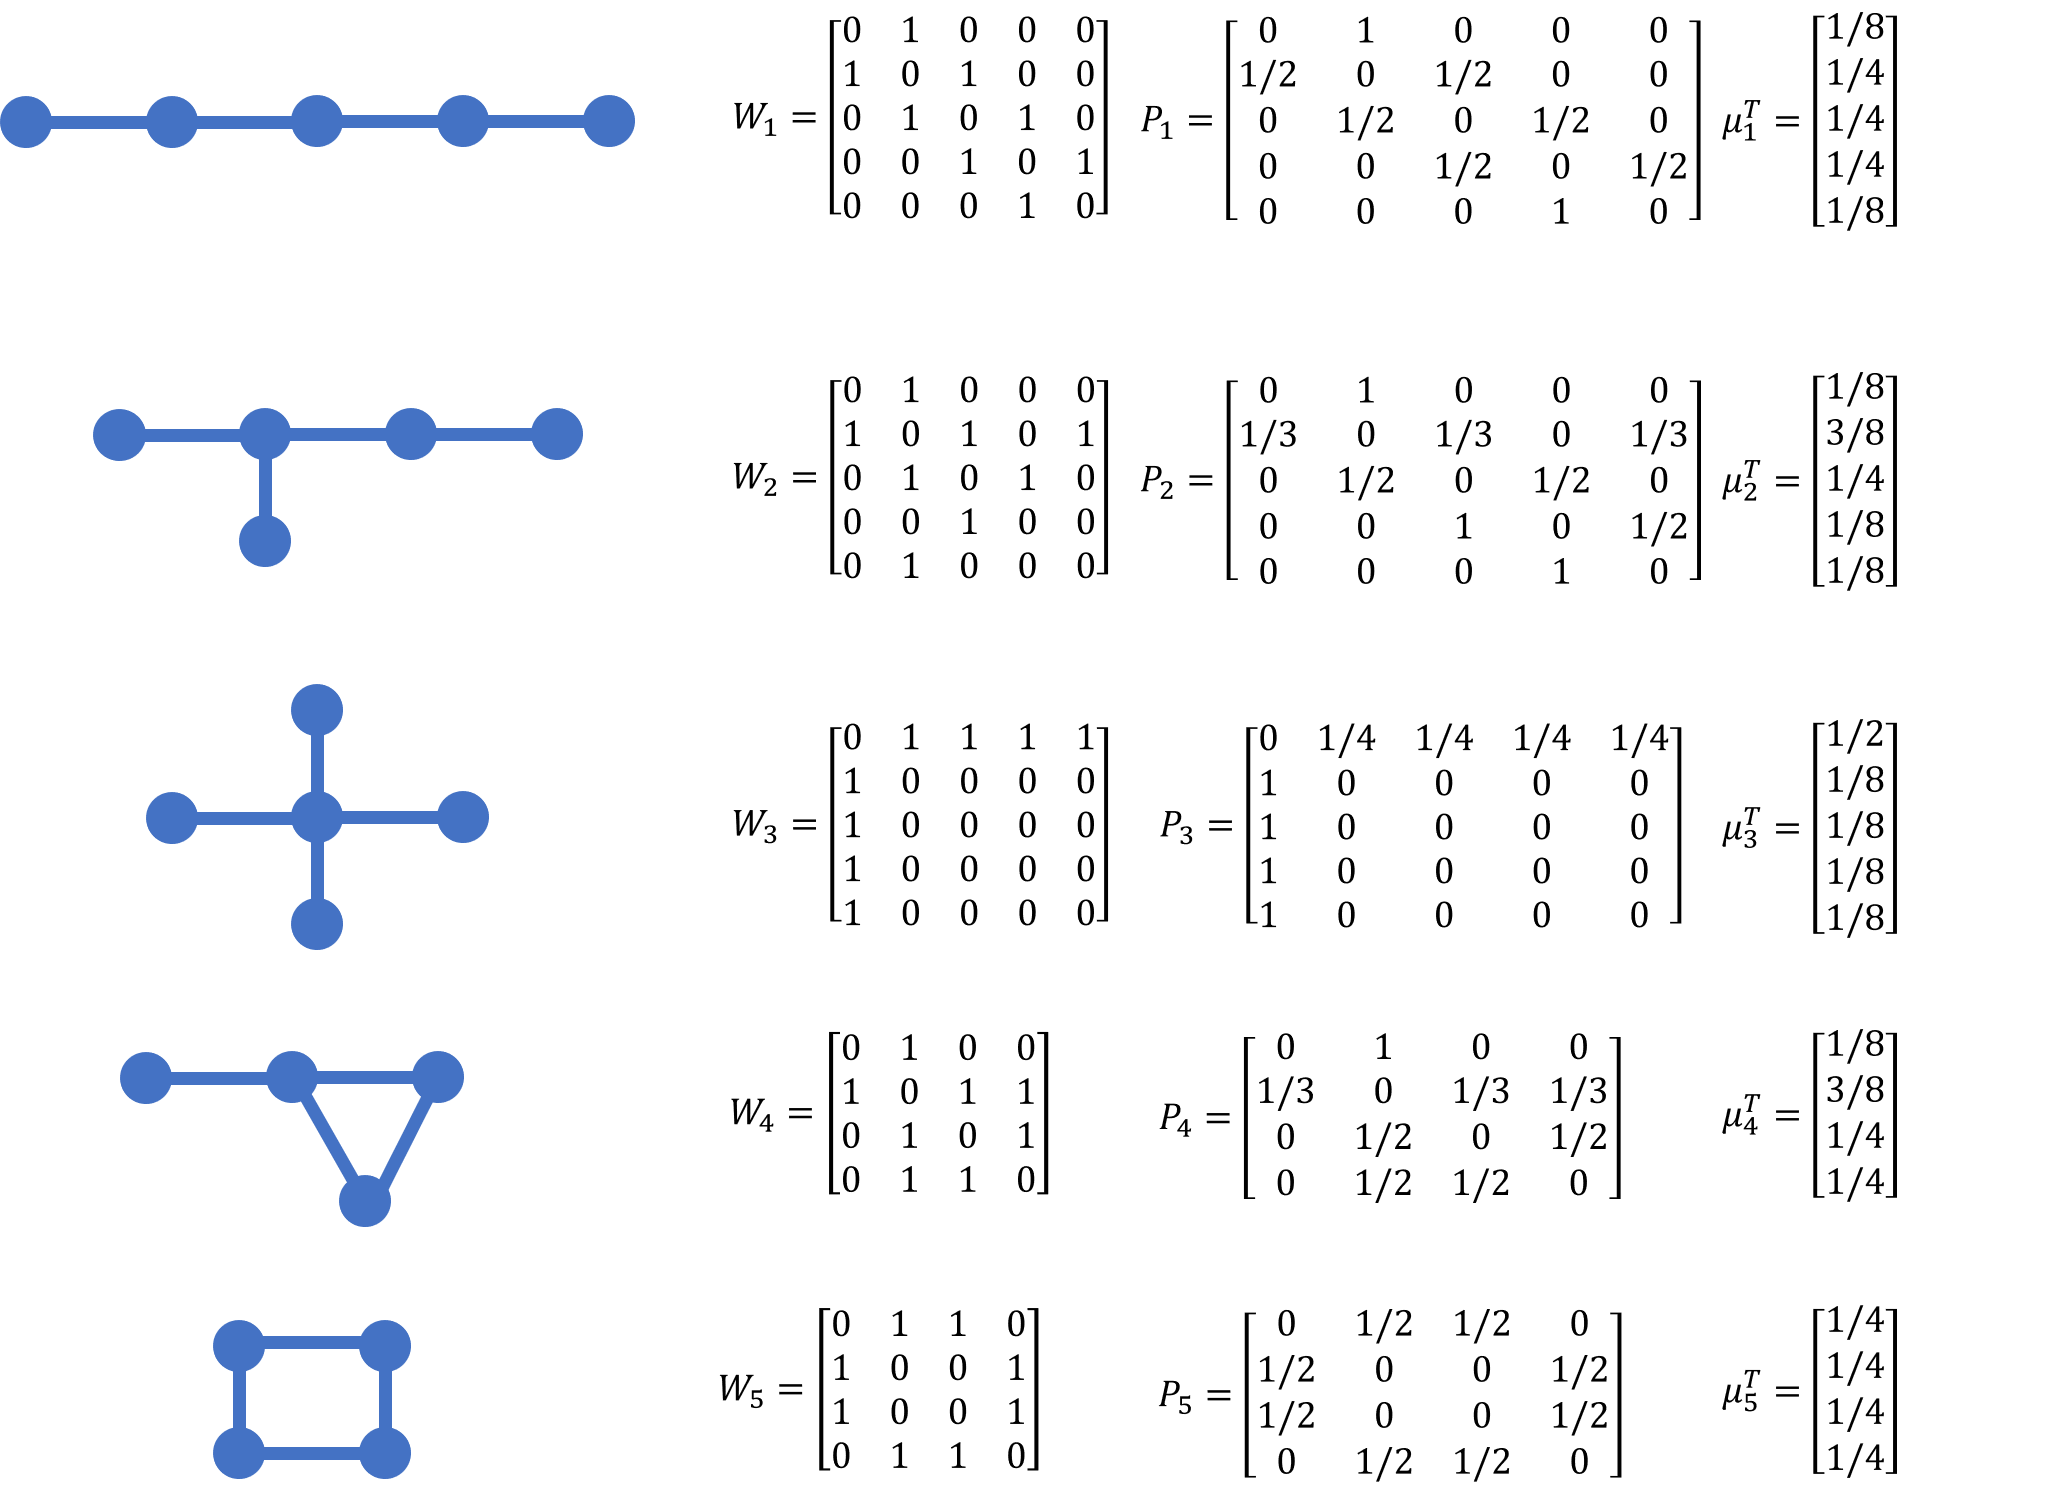
\includegraphics[width=16cm]{img/4-1.png}
        \caption{Five Possible Graphs for Four Edges}
        \label{fig:ex11}
      \end{figure}

      Their corresponding entropy rates are 0.75, 0.84436, 1, 1.09436 and 1.
  \begin{enumerate}
    \item {
    The fourth graph has the largest entropy rate.
    }
    \item { The first graph has the lowest entropy rate.
    }
  \end{enumerate}
  \end{solution}
  \label{ex11}
\end{exercise}

\end{document}
